\documentclass[tikz]{standalone} 
\usepackage{tikz} 
\usepackage{amsmath, amssymb} 
\usetikzlibrary{shapes.multipart} 
\begin{document} 
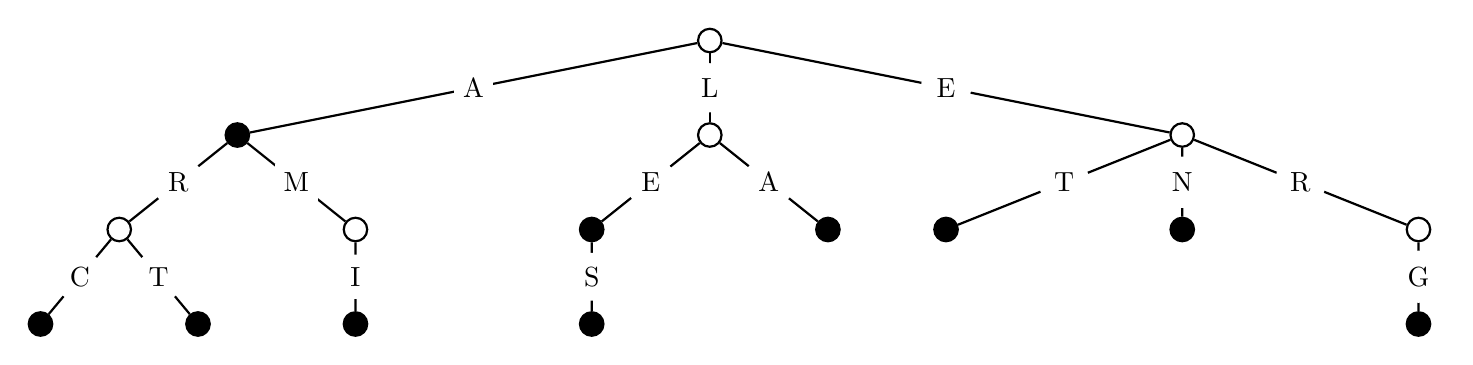
\begin{tikzpicture}[
  thick,
  tree node/.style={
    draw, circle, inner sep = 3pt, 
  },
  edge node/.style={
    draw=none, fill=white, circle, inner sep = 3pt, 
  },
  final/.style={
    fill=black, 
  },
  level/.style={
    sibling distance=60mm/#1, 
    level distance=12mm
  }
  ]
  \draw (0,0) node[tree node] {}
    child {
      node[tree node, final] {}
      child {
        node[tree node] {}
        child {
          node[tree node, final]{} edge from parent node[edge node] {C}
        }
        child {
          node[tree node, final] {} edge from parent node[edge node] {T}
        }
        edge from parent node[edge node] {R}
      }
      child {
        node[tree node] {}
        child {
          node[tree node, final] {}
          edge from parent node[edge node] {I}
        }
        edge from parent node[fill=white] {M}
      }
      edge from parent node[fill=white] {A}
    }
    child {
      node[tree node] {}
      child {
        node[tree node, final] {}
        child{
          node[tree node, final] {}
          edge from parent node[edge node] {S}
        }
        edge from parent node[edge node] {E}
      }
      child {
        node[tree node, final] {}
        edge from parent node[edge node] {A}
      }
      edge from parent node[edge node] {L}
    }
    child {
      node[tree node] {}
      child {
        node[tree node, final] {}
        edge from parent node[edge node] {T}
      }
      child {
        node[tree node, final] {}
        edge from parent node[edge node] {N}
      }
      child {
        node[tree node] {}
        child {
          node[tree node, final] {}
          edge from parent node[edge node] {G}
        }
        edge from parent node[edge node] {R}
      }
      edge from parent node[edge node] {E}
    }
; 
\end{tikzpicture}

\end{document}
